
\begin{lem}\label{片方}
Let $\sharp \Sigma \ge 3$ and $p,~q$ regular patterns on $\Sigma$.
Suppose that the finite set $D$ of regular patterns is one of the following {\rm (i), (ii)}.
Then, if $p \{ x := r \} \preceq q$ for all $r \in D$, then $p \{ x := xy \} \preceq q$.
\begin{enumerate}
\item[{\rm (i)}] $D=\{ ya, bc, dy \}$ $(b = a,~c \not = a,d,\mbox{~and~} b \not = d)$,
\item[{\rm (ii)}] $D=\{ ya, bc, dy \}$ $(b \not = a,d,~c = d,\mbox{~and~} c \not = a)$.
\end{enumerate}
\end{lem}
\begin{proof}

It is obvious if no variable symbol appears in $p$.
Therefore, let $p=p_{1}xp_{2}$ ($p_{1}, p_{2}$ are regular patterns and $x$ is a variable symbol). Assume that $p \{ x := xy \} \not \preceq q$ and derive the contradiction.

\noindent\textrm{(i)}
Let $D=\{ ya, bc, dy \}$ $(b = a,~c \not = a,d,\mbox{~and~}b \not = d)$.
Since $p \{ x := r \} \preceq q$ for all $r \in D$, there are three strings of length $2$ corresponding to $ya, bc, dy$ in $q$. Note that the three strings may appear partly overlapping.
The symbols appearing in $D$ corresponds to a variable or a constant in $q$.
Let $y_{1}, y_{2}, y_{3}$ be variable symbols appearing in $q$.
The strings $ya$ and $dy$ must correspond to the strings $y_{1}a$ and $dy_{3}$ in $q$, respectively.
There are the following three possibilities of strings in $q$ which corresponds to $bc$ in $p\{x:=bc\}$.
\begin{center}
\begin{tabular}{cccccc}
\textrm{(a)} & $bc$, &
\textrm{(b)} & $y_{2}c$, &
\textrm{(c)} & $by_{2}$.
\end{tabular}
\end{center}

\textrm{(a)}
Let $A,B,C$ be strings where $\{ A,B,C \} = \{ y_{1}a,bc,dy_{3} \}$ and let $q=q_{1}AwBw^{\prime}Cq_{2}$.
Since $p \{ x := r \} \preceq q$ for all $r \in D$ and $p \{ x := xy \} \not \preceq q$ hold, the following conditions hold:
\begin{align*}
(1)~& p_{1} \preceq q_{1} & (1')~& p_{2} \preceq wBw^{\prime}Cq_{2} \\
(2)~& p_{1} \preceq q_{1}Aw & (2')~& p_{2} \preceq w^{\prime}Cq_{2} \\
(3)~& p_{1} \preceq q_{1}AwBw^{\prime} & (3')~& p_{2} \preceq q_{2}
\end{align*}

Let $q^{\prime}_{1}=q_{1}A,~q^{\prime}_{2}=wBw^{\prime},~q^{\prime}_{3}=Cq_{2}$. From $(3)$ and $(1')$, we have $p_{1} \preceq q^{\prime}_{1}q^{\prime}_{2},~p_{2} \preceq q^{\prime}_{2}q^{\prime}_{3}$.
From Lemma \ref{補題9}, if $q^{\prime}_{2}$ contains a variable, $p \preceq q$ holds.
Therefore, $B$ must be $bc$.
If $A=dy_{3}$, from $(2)$, $p_{1} \preceq q_{1}dy_{3}w$ holds.
Let $p_{1}=p^{\prime}_{1}p^{\prime\prime}_{1}, p^{\prime}_{1} \preceq q_{1}d$, and $p^{\prime\prime}_{1} \preceq y_{3}w$.
From $(1')$, we have $p=p_{1}xp_{2}=p^{\prime}_{1}p^{\prime\prime}_{1}xp_{2} \preceq q_{1}dp^{\prime\prime}_{1}xwbcw^{\prime}y_{1}aq_{2}=q \{ x:=p^{\prime\prime}_{1}x \}$. This shows that there is a substitution $\theta$ such that $p=q\theta$ holds, and this contradicts the assumption. Therefore, we only need to consider the case where $A=y_{1}a,B=bc$, and $C=dy_{3}$.

From the above, we consider two cases: one in which the symbols overlap and the other in which they do not.
\smallskip

\begin{tabular}{cl}
\textrm{(a-1)} & $q=q_{1}y_{1}awbcw^{\prime}dy_{3}q_{2}$,\\
\textrm{(a-2)} & $q=q_{1}y_{1}acwdy_{3}q_{2}$~~($a=b$).
\end{tabular}
\smallskip

\textrm{(a-1)}
From the proof of Lemma \ref{追加部分}, $p \{ x:= xy \} \preceq q$ holds.
Therefore, it contradicts the assumption.

\textrm{(a-2)}
Let $q=q_{1}y_{1}acwdy_{3}q_{2}$ ($a=b$).
For this $q$, the following conditions hold:
\begin{align*}
(1)~& p_{1} \preceq q_{1} & (1')~& p_{2} \preceq cwdy_{3}q_{2} \\
(2)~& p_{1} \preceq q_{1}y_{1} & (2')~& p_{2} \preceq wdy_{3}q_{2} \\
(3)~& p_{1} \preceq q_{1}y_{1}acwdy_{3} & (3')~& p_{2} \preceq q_{2}
\end{align*}

%
If $|w|=0$, from $(1')$ and $(2')$, the prefix of $p_{2}$ is $cd$ and $d$.
Therefore, $c=d$. This contradicts the fact that $c \not = d$.

If $|w|=1$, from (1') and (2'), the prefix of $p_{2}$ is $cwd$ and $wd$.
Therefore, $w=c=d$.
This contradicts the fact that $c \not = d$.

If $|w| \ge 2$, then from $(1')$ and $(2')$,  prefixes of $p_{2}$ is $cwd$ and $wd$.
Let $w$ be $w_{1}w_{2}w_{3} \cdots w_{n-1}w_{n}$ $(n\geq 2,~w_{i}\in\Sigma$ for $i=1, \ldots , n)$.
From $cw=wd$, a prefix of $w$ is $c$ and a suffix of $w$ is $d$.
Therefore, we have $w=cw_{2}w_{3} \cdots w_{n-1}d$.
Since $cw=cw_{2}w_{3} \cdots w_{n-1}d,~wd=cw_{2}w_{3} \cdots w_{n-1}dd$, from $cw=wd$, $w_{i}=w_{i+1}$ holds for $i=2, \ldots , n-2$.
Therefore, $c=d$. This contradicts the fact that $c \not = d$.

\textrm{(b)}
Let $q=q_{1}AwBw^{\prime}Cq_{2}$ where $\{ A,B,C \} = \{ y_{1}a,y_{2}c,dy_{3} \}$, and let $q=q_{1}AwBw^{\prime}Cq_{2}$.
Since $c \not = a$ holds, $q$ have a substring that is corresponding to (i-2) of Lemma~\ref{変数2つ}.
Therefore, $p \{ x:= xy \} \preceq q$ holds.
This contradicts the assumption. 

\textrm{(c)} As in (b), this contradicts the assumption.

\noindent\textrm{(ii)}
In this case, by reversing the strings $p$ and $q$, we can prove that the assumption $p \{ x := xy \} \preceq q$ is contradicted, as in the case of \textrm{(i)}.
\end{proof}

From Lemmas \ref{追加部分} and \ref{片方}, we obtain the following corollary:

\begin{col}\label{両方}
  Let $\sharp \Sigma \ge 3$ and $p, q$ regular patterns on $\Sigma$.
  For a variable symbol $y$, if $D= \{ ya, bc, dy \}$ $(b = a$ and $c = d)$, there exists $q$ such that $p \{ x := r \} \preceq q$ for any $r \in D$, then $p \{ x := xy \} \not \preceq q$.
\end{col}
\begin{ex}
Let $a,b,c,d,e$ be constant symbols in $\Sigma$ and 
$x,y,y_{1},y_{2}$ variable symbols.
Let 
\begin{align*}
p &= eabcbcadabcbcadaxbcadadabcbcadade,\\
q &= y_{1}abcbcadabcbcadady_{2}~~~~~(b = a\mbox{~and~}c = d).
\end{align*}

\noindent
Obviously $p \{ x:=xy \} \not \preceq q$ holds.
For these $p$ and $q$, the condition for Corollary \ref{両方} holds as follows (see also Fig.~\ref{b=aとc=dの例}):
\begin{eqnarray*}
&p& \{ x:=ya \} \\ 
& = & (eabcbcadabcbcaday)abcadadabcbcadade\\
& = & q \{ y_{1} := eabcbcadabcbcaday,~y_{2}:=e \} \\
& \preceq & q,\\
&p& \{ x:=bc \}  \\
& = & (eabcbcad)abcbcadabcbcadad(abcbcadade) \\
& = & q \{ y_{1} := eabcbcad,~y_{2} := abcbcadade \} \\
& \preceq & q,\\
&p& \{ x:=dy \}  \\
& = & eabcbcadabcbcadad(ybcadadabcbcadade) \\
& = & q \{ y_{1}:=e,~y_{2} := ybcadadabcbcadade \} \\
& \preceq & q.
\end{eqnarray*}
\end{ex}

\begin{figure}[t]
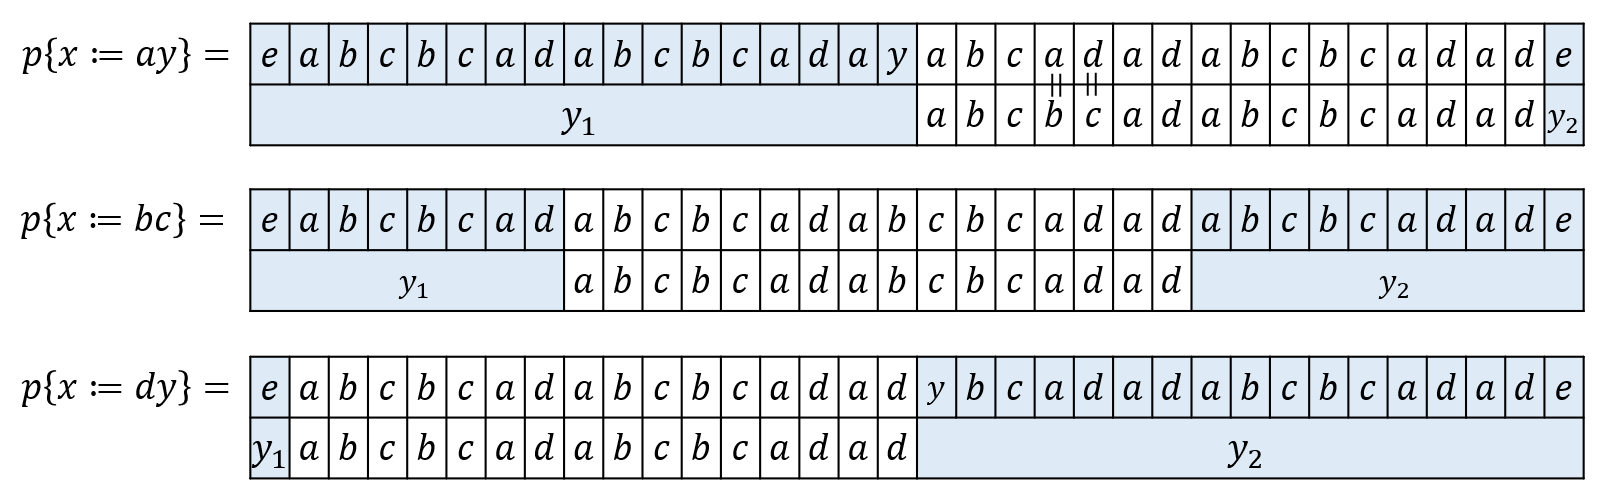
\includegraphics[width=\linewidth]{figs/Exam_b=a_c=d.png}
\caption{Substitutions for $p$ and each correspondence to $q$.}
\label{b=aとc=dの例}
\end{figure}

\begin{comment}
\begin{lem}\label{追加補題2}
Let $\sharp \Sigma \ge 3$ and $p, q$ regular patterns on $\Sigma$.
Let $D= \{ ya,ab,by,cd \}$ $(cd \not = ab)$ be a set consisting of constant symbols $a,b,c,d$ in $\Sigma$ and a variable symbol $y$.
If for all $r \in D$, $p \{ x := r \} \preceq q holds, then $p \{ x := xy \} \preceq q$ holds.
\end{lem}
\begin{proof}
$p$に変数記号が現れない場合は自明である.
したがって,$p=p_{1}xp_{2}$ ($p_{1}, p_{2}$は正規パターン, $x$は変数記号)とおく.$p \{ x := xy \} \not \preceq q$と仮定して,矛盾を導く.

$c \not = a$かつ$d \not = b$であるとき,系\ref{両方}より,$p \{ x:= xy \} \preceq q$となる.
これは,仮定に矛盾する.

$c \not = a$かつ$d = b$,または,$c = a$かつ$d \not = b$であるとき,補題\ref{片方}より,$p \{ x:=xy \} \preceq q$となる.
これは,仮定に矛盾する.
\end{proof} 
\end{comment}
%\begin{lem}\label{追加補題1}
%$k \ge 3$,$m \ge \sqrt{k+1}$,$\sharp \Sigma \ge k+m$,$P \in \RPatplus$,$Q \in \RPat^{k}$とする.
%すべての定数記号$a, b \in \Sigma$に対し,ある正規パターン$q \in Q$が存在し,
%$p \{ x:=ab \} \preceq q$ならば,$p \{ x:=xy \} \preceq q$となる.
%\end{lem}

\begin{lem}\label{追加補題1}
Let $k$ be an integer with $k\geq 1$.
Let $\Sigma$ be an alphabet with $\sharp \Sigma = k + 2$.
Let $p \in \RPat$ in which a variable symbol $x$ appears, and let $Q \in \RPat^{k}$.
If for any string $w \in \Sigma^{\ast}$ with $|w|=2$, there exists a regular pattern $q_{w} \in Q$ such that $p \{ x:=w \} \preceq q_{w}$ holds, then there exists a regular pattern $q \in Q$ such that $p \{ x:=xy \} \preceq q$ holds.
\end{lem}

\begin{proof}
For any $q \in Q$, we define the sets $A(q), B(q) \subset \Sigma$ as follows:
\begin{align*}
  A(q) & = \{ a \in \Sigma \mid p \{ x:=ay \} \preceq q,\ y\in X\},\\ 
  B(q) & = \{ b \in \Sigma \mid p \{ x:=yb \} \preceq q,\ y\in X\}.
  \end{align*}
  If there exists $q\in Q$ such that $|A(q)|\geq 2$ or $|B(q)|\geq 2$, from Lemma~\ref{変数2つ}, $p\{x := xy\} \preceq q$ holds.
Suppose that $|A(q)|\leq 1$ and $|B(q)|\leq 1$.
Let $\varnothing$ be a constant symbol that is not a member in $\Sigma$.
We define the functions $\sigma_{A}: Q \rightarrow \Sigma \cup \{\varnothing\}$ and $\sigma_{B}: Q \rightarrow \Sigma \cup \{\varnothing\}$ as follows:
\begin{align*}
  \sigma_{A}(q) & =
  \begin{cases}
    a & \textrm{if } A(q) = \{a\}, \\
    \varnothing & \textrm{if } A(q) = \emptyset.
  \end{cases}\\
  \sigma_{B}(q) & =
  \begin{cases}
    b & \textrm{if } B(q) = \{b\}, \\
    \varnothing & \textrm{if } B(q) = \emptyset.
  \end{cases}
\end{align*}
We use the following notations that denote the subsets of $\Sigma$:
\begin{align*}
  A & = \bigcup_{q \in Q \textrm{~s.t.~}\sigma_{A}(q) \not= \varnothing} A(q),\\
  B & = \bigcup_{q \in Q \textrm{~s.t.~}\sigma_{B}(q) \not= \varnothing} B(q),\\
  A' & = \Sigma \setminus A, \mbox{ and } B' = \Sigma \setminus B.
\end{align*}
For any $a,b \in \Sigma$, we define the following notations:
\begin{align*}
  \ell_{A}(a) & = \{ q \in Q \mid p \{ x:=ay \} \preceq q,\ y\in X\},\\ 
  \ell_{B}(b) & = \{ b \in \Sigma \mid p \{ x:=yb \} \preceq q,\ y\in X\}\\
  \ell_{A} &= \sum_{a \in \Sigma}(\ell_{A}(a) - 1),\\
  \ell_{B} &= \sum_{b\in \Sigma}(\ell_{B}(b) - 1),
\end{align*}
We easily see the following claim:  

\smallskip

\noindent
\textit{Claim} 1. 
\begin{enumerate}
  \item[(i)] $\ell_{A} = k - \sharp \sigma_{A}^{-1}(\varnothing) - \sharp A$, and
  \item[(ii)] $\ell_{B} = k - \sharp \sigma_{B}^{-1}(\varnothing) - \sharp B$,
\end{enumerate}
where $\sigma_{A}^{-1}$ and $\sigma_{B}^{-1}$ are the inverse functions of $\sigma_{A}$ and $\sigma_{B}$, respectively.

\smallskip

Since $\sharp \Sigma = k + 2$ and $\sharp Q = k$, $\sharp A' \geq 2$ and $\sharp B' \geq 2$ hold.
Moreover, we use the following notations that denote the subsets of $Q$:
\begin{align*}
  Q^{(\varnothing,\varnothing)} & = \{q \in Q \mid \sigma_{A}(q) = \varnothing \textrm{~and~} \sigma_{B}(q) = \varnothing\},\\
  Q^{(\varnothing,\cdot)} & = \{q \in Q \mid \sigma_{A}(q) = \varnothing \textrm{~and~} \sigma_{B}(q) \not= \varnothing\},\\
  Q^{(\cdot,\varnothing)} & = \{q \in Q \mid \sigma_{A}(q) \not= \varnothing \textrm{~and~} \sigma_{B}(q) = \varnothing\},\\
  Q^{(\cdot,\cdot)} & = \{q \in Q \mid \sigma_{A}(q) \not= \varnothing \textrm{~and~} \sigma_{B}(q) \not= \varnothing\}.
\end{align*}
Suppose that for any string $w \in \Sigma^{\ast}$ with $|w|=2$, there exists a regular pattern $q_{w} \in Q$ such that $p \{ x:=w \} \preceq q_{w}$ holds.
It is easy to see that if $w \in (A\cdot B) \cup (A'\cdot B) \cup (A\cdot B')$, there exists a regular pattern $q_{w} \in Q^{(\varnothing,\cdot)} \cup Q^{(\cdot,\varnothing)} \cup Q^{(\cdot,\cdot)}$ such that $p \{ x:=w \} \preceq q_{w}$ holds.

For $w=a'b'\in A'\cdot B'$, we must have $q_{w} \in Q$ that satisfies that $p \{ x:=w \} \preceq q_{w}$. The following two claims are proven from Lemmas~\ref{変数2つ} and \ref{補題14}:

\smallskip

\noindent
\textit{Claim} 2. If there exist $q \in Q^{(\varnothing,\varnothing)}$ and distinct $5$ strings $w_{i} \in A'\cdot B'$ ($1\leq i\leq 5$) such  that $p \{ x:=w_{i} \} \preceq q$ holds ($1\leq i\leq 5$),  then $p \{ x:=xy \} \preceq q$ holds.

\smallskip

\noindent
\textit{Claim} 3. If there exist $q \in Q^{(\varnothing,\cdot)} \cup Q^{(\cdot,\varnothing)}$ and distinct $3$ strings $w_{i} \in A'\cdot B'$ ($1\leq i\leq 3$) such that $p \{ x:=w_{i} \} \preceq q$ holds ($1\leq i\leq 3$),  then $p \{ x:=xy \} \preceq q$ holds.

\smallskip

\noindent
Assume that the conditions of \textit{Claims} 2 and 3 are not satisfied.
Let ${\cal L}_{1}$ be the number of the strings $w \in A'\cdot B'$ such that there exists a regular pattern $q_{w} \in Q^{(\varnothing,\varnothing)} \cup Q^{(\varnothing,\cdot)} \cup Q^{(\cdot,\varnothing)}$ such that $p \{ x:=w \} \preceq q_{w}$ holds.
Then, by \textit{Claim} 1,
\begin{align*}
  {\cal L}_{1} &\leq 4\sharp Q^{(\varnothing,\varnothing)} + 2\sharp Q^{(\varnothing,\cdot)} + 2\sharp Q^{(\cdot,\varnothing)}\\
  & = 2(Q^{(\varnothing,\varnothing)} + \sharp Q^{(\varnothing,\cdot)}) + 2(Q^{(\varnothing,\varnothing)} + \sharp Q^{(\cdot,\varnothing)})\\
  & = 2\sharp \sigma_{A}^{-1}(\varnothing) + 2\sharp \sigma_{B}^{-1}(\varnothing)\\
  & = 2(k - \ell_{A} - \sharp A) + 2(k - \ell_{B} - \sharp B)\\
  & = 2(\sharp A' - \ell_{A} - 2) + 2(\sharp B' - \ell_{B} - 2)\\
  & = 2(\sharp A' + \sharp B') - 2(\ell_{A} + \ell_{B}) - 8.
\end{align*}
  
Next, we show the next two claims:

\smallskip

\noindent
\textit{Claim} 4. 
For constant symbols $a \in A$, $a' \in A'$, $b \in B$, $b' \in B'$ such that $p\{x:=yb\} \preceq q$, $p\{x:=a'b'\} \preceq q$, and $p\{x:=ay\} \preceq q$ hold,
if $a \in A\cap B$ or $b \in A\cap B$, then $p\{x:=xy\} \preceq q$ holds.

\smallskip

\noindent
\textit{Proof of Claim} 4. 
When both $a\in A\cap B$ and $b \in A\cap B$ hold, since $a' \not= a, b$ and $b' \not= a, b$, from Lemma~\ref{追加部分}, $p\{x:=xy\} \preceq q$ holds.
Suppose that $a\in A\cap B$ and $b\in A'\cap B$.
If $a' = b$, since $a\in A\cap B$ and $a' \in A'\cap B$, $b' \not= a, a'$ holds, and therefore from Lemma~\ref{片方}, $p\{x:=xy\} \preceq q$ holds. If $a' \not= b$, since $b' \not\in A\cap B$, $b' \not= a$ holds, and therefore from Lemma~\ref{追加部分}, $p\{x:=xy\} \preceq q$ holds.
In the case of $a\in A\cap B'$ and $b\in A\cap B$, the statement is similarly proven. (\textit{End of Proof of Claim})

\smallskip

\noindent
\textit{Claim} 5. 
For constant symbols $a \in A$, $a' \in A'$, $b \in B$, $b' \in B'$ such that $p\{x:=yb\} \preceq q$, $p\{x:=a'b'\} \preceq q$, and $p\{x:=ay\} \preceq q$ hold, if the following conditions (i) and (ii) are satisfied, then $p\{x:=xy\} \preceq q$ holds.
\begin{enumerate}
  \item[(i)] $a \in A\cap B'$ and $b \in A'\cap B$,
  \item[(ii)] $a' \not= b$ or $b' \not= a$.
  \end{enumerate}
  
  \smallskip

  \noindent
  \textit{Proof of Claim} 5. 
  When $a'=b'$, since $a \not= b$, from Lemma~\ref{追加部分}, this statement holds. When $a' \not = b'$, since $a \not= b$, from Lemma~\ref{追加部分} or Lemma~\ref{片方}, this holds.  (\textit{End of Proof of Claim})
  
  \smallskip
  
Assume that the conditions of \textit{Claims} 4 and 5 are not satisfied.
I.e., for constant symbols $a \in A$, $a' \in A'$, $b \in B$, $b' \in B'$ such that $p\{x:=yb\} \preceq q$, $p\{x:=a'b'\} \preceq q$, and $p\{x:=ay\} \preceq q$ hold, the next conditions are assumed:
\begin{enumerate}
\item $a \in A\cap B'$ and $b \in A'\cap B$,
\item $a' = b$ and $b' = a$.
\end{enumerate}

\noindent
Let ${\cal L}_{2}$ be the number of the strings $w=a'b' \in A'\cdot B'$ such that there exists a regular pattern $q_{w} \in Q$ such that $A(q_{w})=\{b'\}=\{a\}$, $B(q_{w})=\{a'\}=\{b\}$, and $p \{ x:=w \} \preceq q_{w}$ holds. Considering the duplicate numbers $\ell_{A}$ and $\ell_{B}$,

We show the last claim:
  
\smallskip

\noindent
\textit{Claim} 6. 
$\sharp A' \times \sharp B' - {\cal L}_{1} - {\cal L}_{2} > 0$.

\smallskip

\noindent
\textit{Proof of Claim} 6. 
First we prove the inequality when $\sharp A \leq k - 1$ and $\sharp B \leq k - 1$, i.e., $\sharp A' \geq 3$ and $\sharp B' \geq 3$ hold.
Since ${\cal L}_{2} \leq \frac{1}{2}(\sharp A' + \sharp B' + \ell_{A} + \ell_{B})$,
\begin{align*}
  &\ \sharp A' \times \sharp B' - {\cal L}_{1} - {\cal L}_{2}\\
\geq &\ \sharp A' \times \sharp B' - (2(\sharp A' + \sharp B') - 2(\ell_{A} + \ell_{B}) - 8)\\
  &\ - \frac{1}{2}(\sharp A' + \sharp B' + \ell_{A} + \ell_{B})\\
=    &\ \sharp A' \times \sharp B' - \frac{5}{2}(\sharp A' + \sharp B') + \frac{3}{2}(\ell_{A} + \ell_{B}) + 8\\
=    &(\sharp A' - \frac{5}{2})(\sharp B' - \frac{5}{2}) + \frac{3}{2}(\ell_{A} + \ell_{B}) + \frac{7}{4} > 0.
\end{align*}
When $\sharp A = k$ and $\sharp B \leq k$, i.e., $\sharp A' = 2$ and $\sharp B' \geq 2$ hold, since $\ell_{A} = 0$,
${\cal L}_{1} \leq 2\sharp B' - 2\ell_{B} -4$ holds.
Moreover, ${\cal L}_{2} \leq \min\{\sharp B', \ell_{B} + 2\}$ holds.
From \textit{Claim} 1, $\ell_B + 2 = k - \sharp\sigma^{^1}_{B}(\varnothing) - \sharp B = \sharp B' - \sharp\sigma^{^1}_{B}(\varnothing)$ hold. Therefore, ${\cal L}_{2} \leq \ell_{B} + 2$ holds.
Thus,
\begin{align*}
  &\ \sharp A' \times \sharp B' - {\cal L}_{1} - {\cal L}_{2}\\
\geq &\ 2\sharp B' - (2\sharp B' - 2\ell_{B} -4) - (\ell_{B} + 2)\\
= & \sharp B' + \ell_B + 2 > 0.
\end{align*}
Similarly, the case when $\sharp A \leq k$ and $\sharp B = k$ is proven.
(\textit{End of Proof of Claim})

\smallskip

From \textit{Claim} 6, there exist $w\in A'\cdot B'$ and a regular pattern $q_{w} \in Q$ such that either of the conditions of \textit{Claims} 2--5 is satisfied. 
Therefore, for such a regular pattern $q_{w}$, $p \{x := xy\} \preceq q_{w}$ holds.
\end{proof}

\begin{lem}[Sato et al.\cite{Sato1}]\label{補題15}
Let $\Sigma$ be a finite alphabet with $\sharp \Sigma \ge 3$ and $p,q$ be regular patterns.
If there exists a constant symbol $a \in \Sigma$ such that $p \{ x := a \} \preceq q$ and $p \{ x := xy \} \preceq q$, then $p \preceq q$ holds, where $y$ is a variable symbol that does not appear in $q$.
\end{lem}

\hfill Edited by Takayoshi Shoudai.
\hrule
\bigskip

%補題\ref{追加補題1},補題\ref{補題15}より,次の定理が成り立つ.

\begin{thm}\label{定理17}
$k \ge 3$,$\sharp \Sigma \ge 2k-1$,$P \in \RPatplus,Q \in \RPat^{k}$とする.
このとき,以下の{\rm (i),(ii),(iii)}は同値である.
\[
\begin{tabular}{ll}
$(\mathrm{i})$ $S_{2}(P) \subseteq L(Q),$
$(\mathrm{ii})$ $P \sqsubseteq Q,$
$(\mathrm{iii})$ $L(P) \subseteq L(Q).$
\end{tabular}
\]
\end{thm}

\begin{proof}
(ii) $\Rightarrow$ (iii)と(iii) $\Rightarrow$ (i)は自明である.
定理\ref{定理10}より,$\sharp\Sigma \ge 2k+1$のとき,(i) $\Rightarrow$ (ii)は成り立つ.
よって,$\sharp Q=k$のとき,$\sharp\Sigma = 2k-1$または$\sharp\Sigma = 2k$の場合,(i) $\Rightarrow$ (ii)が成り立つことを,$p$に含まれる変数記号の数$n$に関する数学的帰納法により証明する.

$n=0$のとき,$S_{2}(p)= \{ p \}$であり,$p \in L(Q)$となる.よって,ある$q \in Q$に対して,$p \preceq q$となる.

$n \ge 0$個の変数記号を含む任意の正規パターンに対して題意が成り立つと仮定する.
$p$を$S_{2}(p) \subseteq L(Q)$を満たす$n+1$個の変数記号を含む正規パターンとする.
$p \not \preceq q_{i}$ ($i=1, \ldots, k$)と仮定する.
$p=p_{1}xp_{2}$ ($p_{1},p_{2}$は正規パターン,$x$は変数記号),$Q=\{ q_{1}, \ldots , q_{k} \}$を考える.
$a, b \in \Sigma$に対して,$p_{a}=p \{ x := a \}$と$p_{ab}=p \{ x := ab \}$とおく.
このとき,$p_{a},p_{ab}$は$n$個の変数記号が含まれ,$S_{2}(p_{a}) \subseteq L(Q)$かつ$S_{2}(p_{ab}) \subseteq L(Q)$が成り立つことに注意する.
帰納法の仮定より,任意の$a,b \in \Sigma$に対して,$p_{a} \preceq q_{i}$かつ$p_{ab} \preceq q_{i^{\prime}}$を満たすような$i, i^{\prime} \le k$が存在する. 
$D_{i}=\{ a \in \Sigma \mid p \{ x:=a \} \preceq q_{i} \}$ \ ($i=1, \ldots, k$)とする.
ある$i$に対して,$\sharp D_{i} \ge 3$であるとき,補題\ref{補題10}より,$p \preceq q_{i}$となる.これは仮定に矛盾する.
よって,$\sharp D_{i} \le 2$ ($i=1, \ldots, k$)となる場合を考える.
$\sharp\Sigma = 2k-1$のとき,任意の$i$に対して,$\sharp D_{i}=2$または$\sharp D_{i}=1$,$\sharp\Sigma = 2k$のとき,任意の$i$に対して,$\sharp D_{i}=2$となる.
$k \ge 3$であるとき,$2k+1 \ge k+2$となる.
よって,補題\ref{追加補題1}より,$p \{ x:=xy \} \preceq q_{i}$となる$i$が存在する.
したがって,補題\ref{補題15}より,$p \preceq q_{i}$となる.
これは仮定に矛盾する.
  
以上より,(i) $\Rightarrow$ (ii)が成り立つ.
\end{proof}

この定理\ref{定理17}より,次の系が得られる.

\begin{col}\label{命題18}
$k \ge 3$,$\sharp\Sigma \ge 2k-1$,$P \in \mathcal{RP}^{+}$とする.このとき,$S_{2}(P)$は$\mathcal{RPL}^{k}$における$L(P)$の特徴集合である.
\end{col}

\begin{lem}[Sato et al.\cite{Sato1}]\label{補題19}
$\sharp\Sigma \le 2k-2$とする.このとき,$\mathcal{RP}^{k}$は包含に関するコンパクト性を持たない.
\end{lem}

\begin{proof}
$\Sigma = \{ a_{1}, \ldots , a_{k-1}, b_{1}, \ldots , b_{k-1} \}$を$(2k-2)$個の定数記号から成る集合,$p, q_{i}$を正規パターン,$w_{i}~(i = 1, \ldots , k-1)$を例\ref{例題1}と同様に定義された記号列とする.
$q_{k} = x_{1}a_{1}w_{1}xyw_{1}b_{1}x_{2}$とする.
例\ref{例題1}で示した通り,$p \{ x := a_{i} \} \preceq q_{i}$かつ$p \{ x := b_{i} \} \preceq q_{i}~(i=1,2, \ldots ,k-1)$であるとき,$S_{1}(p) \subseteq \bigcup^{k-1}_{i=1} L(q_{i})$となる. 
一方で,任意の$w$ $(|w| \ge 2)$に対して,$p \{ x:= w \} \preceq q_{k}$となる. 
すなわち,$L(p) \subseteq L(Q)$である.
しかし,$p \not \preceq q_{i}$であるため,$L(p) \not \subseteq L(q_{i}) (i=1,2, \ldots k)$である.
したがって,$\RPatkei$は包含に関するコンパクト性を持たない.
\end{proof}

定理\ref{定理17}と補題\ref{補題19}より,次の定理が成り立つ.

\begin{thm}
$k \ge 3$とし,$\sharp\Sigma \ge 2k-1$とする.
このとき,$\RPat^{k}$は包含に関してコンパクト性を持つ.
\end{thm}

$k=2$のとき,次の定理が成り立つ.

\begin{thm}\label{補題21}
$\sharp \Sigma \ge 4$とし,$P \in \RPatplus$,$Q \in \RPat^{2}$とする.
このとき,以下の{\rm (i),(ii),(iii)}は同値である.
\[
\begin{tabular}{ll}
$(\mathrm{i})$ $S_{2}(P) \subseteq L(Q),$
$(\mathrm{ii})$ $P \sqsubseteq Q,$
$(\mathrm{iii})$ $L(P) \subseteq L(Q).$
\end{tabular}
\]
\end{thm}

\begin{proof}
(ii) $\Rightarrow$ (iii)と(iii) $\Rightarrow$ (i)は自明に成り立つ.
よって,(i) $\Rightarrow$ (ii)が成り立つことを示す.
$Q= \{ q_{1}, q_{2} \}$とするとき,$p$に含まれる変数記号の数$n$に関する数学的帰納法で示す.\\
\noindent (1) $n=0$のとき,$p$は定数記号列となるので$S_{2}(p)= \{ p \}$となり
(i)より,$p \in L(Q)$となる.
よって,ある$q \in Q$に対して$p \preceq q$となる.\\
\noindent (2) $n=k$個の変数記号を含むすべての正規パターンに対して有効であると仮定する.
そして,$p$を$S_{2}(p) \subseteq L(Q)$を満たす$(n+1)$個の変数記号を含む正規パターンとする.

$p \not \preceq q_{i}$ ($i=1, 2$)と仮定する.
$p=p_{1}xp_{2}$ ($p_{1}, p_{2}$は正規パターン,$x$は変数記号)を考える.
$a, b \in \Sigma$に対して,$p_{a}=p \{ x := a \}$,$p_{ab}=p \{ x := ab \}$とおく.
このとき,$p_{a},p_{ab}$は$n$個の変数記号が含まれ,$S_{2}(p_{a}) \subseteq L(Q)$,$S_{2}(p_{ab}) \subseteq L(Q)$が成り立つことに注意する.
帰納法の仮定より,任意の$a, b \in \Sigma$に対して,$p_{a} \preceq q_{i}, p_{ab} \preceq q_{i^{\prime}}$を満たすような$i, i^{\prime} \le k$が存在する.

ある$i$に対して$\sharp D_{i} \ge 3$のとき,補題\ref{補題10}より,$p \preceq q_{i}$となる.
よって,任意の$i$に対して,$\sharp D_{i} \le 2$となる.
したがって,$\sharp D_{1}=2$かつ$\sharp D_{2}=2$となる場合を考える.

$\sharp \Sigma = k+2$であるとき,$k=2$より,$\sharp \Sigma =4$となる.
よって,補題\ref{追加補題1}より,ある$i$に対して,$p \{ x:=xy \} \preceq q_{i}$となる.
したがって,補題\ref{補題15}より,$p \preceq q_{i}$となる.
これは,仮定に矛盾する.

以上より,(i) $\Rightarrow$ (ii)が成り立つ.
\end{proof}

次の例は,$k = 2$における定理\ref{補題21}の反例である.
\begin{ex}\label{反例thm17}
$\Sigma= \{a, b, c \}$を$3$つの定数記号から成る集合,$p,q_{1},q_{2}$を正規パターン,$x,x^{\prime},x^{\prime\prime}$を変数記号とする.
\begin{eqnarray*}
p = x^{\prime}axbx^{\prime\prime},
q_{1} = x^{\prime}abx^{\prime\prime},
q_{2} = x^{\prime}cx^{\prime\prime}.
\end{eqnarray*}
$w \in \Sigma^{+}$とする.$w$に$c$が含まれるとき,$p \{ x:=w \} \preceq q_{2}$となり,$c$が含まれないとき,$p \{ x:=w \} \preceq q_{1}$となる.
よって,$L(p) \subseteq L(q_{1}) \cup L(q_{2})$である.
しかし,$p \not \preceq q_{1}$かつ$p \not \preceq q_{2}$である.
\end{ex}

定理\ref{補題21}より,次の2つの系が成り立つ.
\begin{col}
$\sharp\Sigma \ge 4$とし,$P \in \RPatplus$とする.
このとき,$S_{2}(P)$は,$\RPatL^{2}$における$L(P)$の特徴集合である.
\end{col}

\begin{col}
$\sharp\Sigma \ge 4$とする.このとき,クラス$\mathcal{RP}^{2}$は包含に関してコンパクト性を持つ.
\end{col}

